\section{Configuração}

Para a realização deste laboratório, foram configurados os dispositivos de rede com o objetivo de permitir a comunicação entre diferentes sub-redes, o gerenciamento pelo SNMP e o acesso à rede externa.

\subsection{Roteadores}
\subsubsection{Roteador ROT-ACME}

No roteador ROT-ACME, utilizando o sistema operacional VyOS, foram configuradas as interfaces de rede física e virtual (VLANs), atribuindo endereços IP para cada segmento da rede. Além disso, foi definida uma rota padrão para encaminhamento de tráfego externo, implementado o SNMP e o NAT, permitindo o gerenciamento de redes e que as redes internas acessem outras redes por meio da interface de saída. As configurações realizadas podem ser observadas no Código~\ref{lst:rotacme}.

\subsubsection{Roteador R1}

No roteador R1, foram configuradas as interfaces de rede com endereçamento dinâmico na interface de acesso externo e endereçamento estático nas interfaces internas. Além disso, foi implementado o protocolo de roteamento dinâmico OSPF, permitindo a troca de rotas entre os roteadores do backbone. Também foi configurado o NAT para possibilitar o acesso à rede externa, bem como a redistribuição de rotas conectadas. Além disso, foi configurado o protocolo SNMP para permitir o gerenciamento do dispositivo. As configurações realizadas podem ser observadas no Código~\ref{lst:rotR1}.

\subsubsection{Roteador R2}
O roteador R2 foi configurado com endereçamento IP em suas interfaces de rede, interligando diferentes sub-redes do backbone. Assim como no R1, foi utilizado o protocolo OSPF para permitir o roteamento dinâmico entre os dispositivos da rede. Foi configurada uma interface de loopback para identificação do roteador no processo de roteamento, além da redistribuição de rotas conectadas. Também foi configurado o protocolo SNMP para permitir o gerenciamento do dispositivo. As configurações realizadas podem ser observadas no Código~\ref{lst:rotR2}.

\subsubsection{Roteador R3}
No roteador R3, foram configuradas as interfaces de rede responsáveis pela interconexão com outras sub-redes do backbone. O protocolo OSPF foi implementado para permitir a comunicação e troca de informações de roteamento com os demais roteadores. Além disso, foi definida uma identificação única por meio de uma interface de loopback, garantindo a correta operação do protocolo. Também foi configurado o protocolo SNMP para permitir o gerenciamento do dispositivo. As configurações realizadas podem ser observadas no Código~\ref{lst:rotR3}.

\subsection{Switches}

\subsubsection{Switch EXOS1}

No switch EXOS1, foram criadas e configuradas as VLANs correspondentes à rede, incluindo a VLAN de gerenciamento. As portas foram configuradas como trunk para permitir a passagem de múltiplas VLANs entre dispositivos e como acesso para conexão de hosts finais. Também foi atribuído um endereço IP para gerenciamento do equipamento, definida uma rota padrão para comunicação externa e a configuração do SNMP. As configurações realizadas podem ser observadas no Código~\ref{lst:exos1}.

\subsubsection{Switch EXOS2}
O switch EXOS2 foi configurado com VLANs associadas aos diferentes setores da rede, com portas configuradas em modo trunk e acesso conforme a necessidade da topologia. As configurações garantem a comunicação adequada entre os dispositivos conectados e a segmentação lógica da rede. Também foi atribuído um endereço IP para gerenciamento do equipamento, definida uma rota padrão para comunicação externa e a configuração do SNMP. As configurações realizadas podem ser observadas no Código~\ref{lst:exos2}.

\subsubsection{Switch EXOS3}
No switch EXOS3, foram realizadas configurações semelhantes às dos demais switches, com a criação de VLANs e associação de portas em modo trunk e acesso. Essa configuração permite a integração do switch à topologia da rede, garantindo a comunicação entre os diferentes segmentos configurados. Por fim, foi atribuído um endereço IP para gerenciamento do equipamento, definida uma rota padrão para comunicação externa e a configuração do SNMP. As configurações realizadas podem ser observadas no Código~\ref{lst:exos3}.

\subsection{Servidor Zabbix}

A configuração do servidor Zabbix foi realizada com base na documentação oficial do Zabbix\cite{zabbix_install}. Inicialmente, foi realizada a configuração do endereço IP estático do servidor por meio do arquivo \texttt{/etc/netplan/01-network-manager-all.yaml}, conforme apresentado no Código \ref{lst:ZabbixServerIp}.

\begin{listing}[H]
\centering
\begin{minted}[
    bgcolor=bgcolor,
    frame=lines,
    breaklines=true,
    breakanywhere=true,
    fontsize=\footnotesize,
]{yaml}

network:
  version: 2
  renderer: networkd

  ethernets:
    ens3:
      dhcp4: no
      addresses:
        - 172.24.30.4/24
      routes:
        - to: default
          via: 172.24.30.254
      nameservers:
        addresses:
          - 8.8.8.8

\end{minted}
\caption{Configuração do IP - Servidor Zabbix}
\label{lst:ZabbixServerIp}
\end{listing}

Após a configuração do endereço IP, foi realizada a instalação do servidor Zabbix seguindo os procedimentos descritos na documentação oficial. Durante a configuração, foram realizadas alterações no arquivo \texttt{/etc/zabbix/zabbix\_server.conf}, conforme apresentado no Código \ref{lst:ZabbixServerConf}.

\begin{listing}[H]
\centering
\begin{minted}[
    bgcolor=bgcolor,
    frame=lines,
    breaklines=true,
    breakanywhere=true,
    fontsize=\footnotesize,
]{yaml}

DBName=zabbix
DBUser=zabbix
DBPassword=zabbix

\end{minted}
\caption{Configuração do arquivo zabbix\_server.conf}
\label{lst:ZabbixServerConf}
\end{listing}

Por fim, os serviços do servidor Zabbix, Nginx e banco de dados foram reiniciados para aplicação das configurações realizadas, conforme mostrado no Código \ref{lst:ZabbixRestart}.

\begin{listing}[H]
\centering
\begin{minted}[
    bgcolor=bgcolor,
    frame=lines,
    breaklines=true,
    breakanywhere=true,
    fontsize=\footnotesize,
]{bash}

sudo systemctl restart zabbix-server
sudo systemctl restart nginx
sudo systemctl restart mysql

\end{minted}
\caption{Reinicialização dos serviços do servidor Zabbix}
\label{lst:ZabbixRestart}
\end{listing}

\subsection{Linux}

\subsubsection{Linux Server}
Para esse dispositivo, foi feita a configuração dos IPs e do DNS por meio do arquivo \textit{/etc/netplan/01-network-manager-all.yaml}. Nesse arquivo, foram adicionadas as configurações mostradas no Código \ref{lst:LinuxServerIp}.

\begin{listing}[H]
\centering
\begin{minted}[
    bgcolor=bgcolor,
    frame=lines,
    breaklines=true,
    breakanywhere=true,
    fontsize=\footnotesize,
]{yaml}

network:
  version: 2
  renderer: networkd

  ethernets:
    ens3:
      dhcp4: no
      addresses:
        - 172.24.10.2/24
      routes:
        - to: default
          via: 172.24.10.254
      nameservers:
        addresses:
          - 172.16.4.2

\end{minted}
\caption{Configuração do IP - Linux Server}
\label{lst:LinuxServerIp}
\end{listing}

Além da configuração do IP, foi feita a instalação do servidor web - Nginx, como mostrado no Código \ref{lst:LinuxServerWeb}.

\begin{listing}[H]
\centering
\begin{minted}[
    bgcolor=bgcolor,
    frame=lines,
    breaklines=true,
    breakanywhere=true,
    fontsize=\footnotesize,
]{bash}

sudo apt install nginx -y

\end{minted}
\caption{Instalação do servidor web - Linux Server}
\label{lst:LinuxServerWeb}
\end{listing}

Por fim, foi instalado o Zabbix Agent, utilizado para monitoramento do dispositivo pelo servidor Zabbix. Após a instalação, foi realizada a configuração do endereço do servidor responsável pela coleta das métricas e a definição do hostname do equipamento.

A configuração foi realizada no arquivo \texttt{/etc/zabbix/zabbix\_agentd.conf}, conforme apresentado no Código \ref{lst:LinuxServerZabbixAgent}.

\begin{listing}[H]
\centering
\begin{minted}[
    bgcolor=bgcolor,
    frame=lines,
    breaklines=true,
    breakanywhere=true,
    fontsize=\footnotesize,
]{yaml}

Server=172.24.30.4
ServerActive=172.24.30.4
Hostname=LinuxServer

\end{minted}
\caption{Configuração do Zabbix Agent - Linux Server}
\label{lst:LinuxServerZabbixAgent}
\end{listing}

Após a configuração, o serviço do agente foi reiniciado para aplicação das alterações realizadas.

\begin{listing}[H]
\centering
\begin{minted}[
    bgcolor=bgcolor,
    frame=lines,
    breaklines=true,
    breakanywhere=true,
    fontsize=\footnotesize,
]{bash}

sudo systemctl restart zabbix-agent
sudo systemctl enable zabbix-agent

\end{minted}
\caption{Inicialização do serviço Zabbix Agent}
\label{lst:LinuxServerZabbixRestart}
\end{listing}

\subsubsection{Linux Desktop}
Para esse dispositivo, foi feita a configuração dos IPs e do DNS por meio do arquivo \textit{/etc/netplan/01-network-manager-all.yaml}. Nesse arquivo, foram adicionadas as configurações mostradas no Código \ref{lst:LinuxDesktopIp}.

\begin{listing}[H]
\centering
\begin{minted}[
    bgcolor=bgcolor,
    frame=lines,
    breaklines=true,
    breakanywhere=true,
    fontsize=\footnotesize,
]{yaml}

network:
  version: 2
  renderer: networkd

  ethernets:
    ens3:
      dhcp4: no
      addresses:
        - 172.24.10.3/24
      routes:
        - to: default
          via: 172.24.10.254
      nameservers:
        addresses:
          - 172.16.4.2

\end{minted}
\caption{Configuração do IP - Linux Desktop}
\label{lst:LinuxDesktopIp}
\end{listing}

Por fim, foi instalado o Zabbix Agent, utilizado para monitoramento do dispositivo pelo servidor Zabbix. Após a instalação, foi realizada a configuração do endereço do servidor responsável pela coleta das métricas e a definição do hostname do equipamento.

A configuração foi realizada no arquivo \texttt{/etc/zabbix/zabbix\_agentd.conf}, conforme apresentado no Código \ref{lst:LinuxDesktopZabbixAgent}.

\begin{listing}[H]
\centering
\begin{minted}[
    bgcolor=bgcolor,
    frame=lines,
    breaklines=true,
    breakanywhere=true,
    fontsize=\footnotesize,
]{yaml}

Server=172.24.30.4
ServerActive=172.24.30.4
Hostname=LinuxDesktop

\end{minted}
\caption{Configuração do Zabbix Agent - Linux Desktop}
\label{lst:LinuxDesktopZabbixAgent}
\end{listing}

Após a configuração, o serviço do agente foi reiniciado para aplicação das alterações realizadas.

\begin{listing}[H]
\centering
\begin{minted}[
    bgcolor=bgcolor,
    frame=lines,
    breaklines=true,
    breakanywhere=true,
    fontsize=\footnotesize,
]{bash}

sudo systemctl restart zabbix-agent
sudo systemctl enable zabbix-agent

\end{minted}
\caption{Inicialização do serviço Zabbix Agent}
\label{lst:LinuxDesktopZabbixRestart}
\end{listing}

\subsection{PC Windows}

Para a configuração do DNS e do IP do PC Windows, foi utilizada a interface do Painel de Controle, como mostrado na Figura \ref{fig:PCWindowsIP}.

\begin{figure}[H]
    \centering
    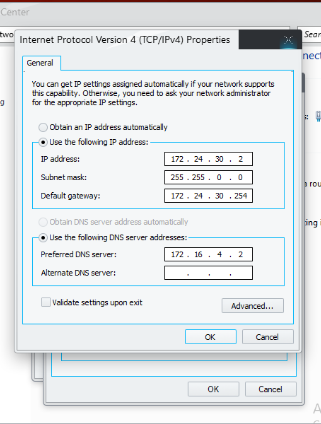
\includegraphics[width=1\linewidth]{fig/PCWindowsIP.png}
    \caption{Configuração IP - PC Windows}
    \label{fig:PCWindowsIP}
\end{figure}

\subsection{VPCs}
Para esse dispositivo, foi feita a configuração dos IPs e do DNS, como mostrado no Código \ref{lst:VPCsIp}.

\begin{listing}[H]
\centering
\begin{minted}[
    bgcolor=bgcolor,
    frame=lines,
    breaklines=true,
    breakanywhere=true,
    fontsize=\footnotesize,
]{bash}

ip 172.24.10.1/24 172.24.10.254
ip dns 172.16.4.2

\end{minted}
\caption{Configuração do IP - VPCs}
\label{lst:VPCsIp}
\end{listing}
